% Task 2: all points from G. Values from Task2/ec_toy.py and the slides (2G from "Doubling G", 3G from Task 1).
% CHECKED (python3, Task2/solution/ec_toy.py): G = (5, 1), 2G = (6, 3), 3G = (10, 6); how many points: not shown
\documentclass[12pt,tikz,border=6pt]{standalone}
% Shared preamble of the task figures of Lecture 5 (based on Lecture02-ChaCha20/task-figures/common.tex).
% The roles take the colours of the elliptic-curves simulator (CryptographySimulators/elliptic-curves),
% so that the README figures and the simulator look the same:
%   secret (number or point): amber, public point: violet, Alice: blue, Bob: green,
%   Eve: red, ciphertext: brown, message: grey, a change or the unknown: orange.
\usepackage{lmodern}
\usepackage[T1]{fontenc}
\renewcommand{\familydefault}{\sfdefault}
\usepackage{amsmath,amssymb}
\usepackage{xcolor}
\usepackage{fontawesome5}
\usetikzlibrary{arrows.meta, calc, positioning, fit, decorations.pathreplacing, backgrounds}

% ---------- template and neutral ----------
\definecolor{DeepBlue}{HTML}{283593}
\definecolor{AccentOrange}{HTML}{EB5A14}
\definecolor{nInk}{HTML}{37474F}
\definecolor{nLine}{HTML}{90A4AE}
\definecolor{nLight}{HTML}{CFD8DC}
\definecolor{nFill}{HTML}{ECEFF1}
\definecolor{aExec}{HTML}{43A047}
\definecolor{aWrite}{HTML}{E53935}

% ---------- roles (the colours of the elliptic-curves simulator) ----------
\definecolor{rPriv}{HTML}{E2A60E}  \definecolor{rPrivBg}{HTML}{FDF3DC}  \definecolor{rPrivText}{HTML}{9A6B00}
\definecolor{rPub}{HTML}{8A5CD8}   \definecolor{rPubBg}{HTML}{F1EAFD}   \definecolor{rPubText}{HTML}{6A3FB8}
\definecolor{rAli}{HTML}{2F6FDB}   \definecolor{rAliBg}{HTML}{E5EDFB}
\definecolor{rBob}{HTML}{2FA84F}   \definecolor{rBobBg}{HTML}{E3F4E8}   \definecolor{rBobText}{HTML}{1E7E4F}
\definecolor{rEve}{HTML}{E5484D}   \definecolor{rEveBg}{HTML}{FDE9E9}
\definecolor{rCip}{HTML}{A8642A}   \definecolor{rCipBg}{HTML}{F7ECE0}
\definecolor{rMsg}{HTML}{BCC4CC}   \definecolor{rMsgBg}{HTML}{EEF1F4}
\definecolor{rChg}{HTML}{D9621C}   \definecolor{rChgBg}{HTML}{FCE8DA}

\tikzset{
  hw/.style={draw=nLine, thick, fill=nFill, text=nInk, rounded corners=3pt, align=center, inner sep=4pt},
  hwmain/.style={draw=nInk, thick, fill=nInk, text=white, rounded corners=3pt, align=center, inner sep=4pt},
  role/.style={draw=#1, thick, fill=#1Bg, text=nInk, rounded corners=3pt, align=center, inner sep=5pt},
  unk/.style={draw=rChg, thick, dashed, fill=white, text=rChg, rounded corners=3pt, align=center, inner sep=5pt,
    font=\bfseries},
  data/.style={-{Stealth}, very thick, nInk},
  note/.style={font=\small, text=nInk},
  person/.style={circle, fill=#1, draw=#1, text=white, minimum size=1.1cm, font=\Large, inner sep=0pt},
}
\newcommand{\personnode}[4]{%
  \node[person=#3] (#1) at (#2) {\faUser};
  \node[font=\small\bfseries, text=#3, below=0.06cm of #1] (#1lbl) {#4};}
\newcommand{\cogbox}[4]{%
  \node[hwmain, minimum width=#4, minimum height=1.1cm] (#1) at (#2) {};
  \node[text=white, font=\large, anchor=west] at ([xshift=0.2cm]#1.west) {\faCogs};
  \node[text=white, font=\small\bfseries] at ([xshift=0.3cm]#1.center) {#3};}

% ---------- the toy curve y^2 = x^3 + 2x + 2 mod 17 (as on the slides) ----------
% CHECKED: python3, all (x, y) with 0 <= x, y < 17 and y^2 = x^3 + 2x + 2 mod 17: these 18 points
\newcommand{\curvepts}{0/6,0/11,3/1,3/16,5/1,5/16,6/3,6/14,7/6,7/11,9/1,9/16,10/6,10/11,13/7,13/10,16/4,16/13}
% the grid of dots, in grid coordinates (1 unit = one step of x or y); draw it inside a scope
\newcommand{\gridbody}{%
  \foreach \x in {0,...,16} \foreach \y in {0,...,16} \fill[nLight] (\x,\y) circle (1.1pt);
  \draw[nLine, thick] (-0.7,-0.7) -- (16.7,-0.7);
  \draw[nLine, thick] (-0.7,-0.7) -- (-0.7,16.7);
  \foreach \v in {0,...,16} {
    \node[font=\tiny, text=gray, anchor=north] at (\v,-0.75) {\v};
    \node[font=\tiny, text=gray, anchor=east] at (-0.75,\v) {\v};
  }
  \node[font=\scriptsize, text=nInk, anchor=west] at (16.8,-0.7) {$x$};
  \node[font=\scriptsize, text=nInk, anchor=south] at (-0.7,16.8) {$y$};
  \foreach \x/\y in \curvepts \fill[nInk] (\x,\y) circle (3pt);}
% mark a point of the grid: \gmark[colour]{x,y}{label}{where the label goes}
\newcommand{\gmark}[4][rPub]{%
  \node[circle, draw=#1, line width=1.2pt, fill=#1, minimum size=9pt, inner sep=0pt] at (#2) {};
  \node[font=\scriptsize\bfseries, text=#1, #4, inner sep=1pt, outer sep=3pt, fill=white, fill opacity=0.85,
    text opacity=1, rounded corners=1pt] at (#2) {#3};}

\begin{document}
\pagecolor{white}
\begin{tikzpicture}[>=Stealth]
  % the curve mod 17
  \node[font=\normalsize\bfseries, text=nInk, anchor=west] at (-0.5,6.15) {$y^2 = x^3 + 2x + 2 \bmod 17$, \ $G = (5, 1)$};
  \begin{scope}[x=0.32cm, y=0.32cm]
    \gridbody
    \draw[rChg, very thick, ->, shorten >=5pt, shorten <=5pt] (5,1) to[bend left=25] node[left, font=\scriptsize\bfseries] {$+G$} (6,3);
    \draw[rChg, very thick, ->, shorten >=5pt, shorten <=5pt] (6,3) to[bend left=25] node[below right, font=\scriptsize\bfseries] {$+G$} (10,6);
    \draw[rChg, very thick, ->, dashed, shorten <=5pt] (10,6) to[bend left=25] (12.6,10.4);
    \node[unk, font=\scriptsize\bfseries, inner sep=3pt] at (13.3,11.4) {4G = ?};
    \gmark{5,1}{$G$}{below right}
    \gmark{6,3}{$2G$}{right}
    \gmark{10,6}{$3G$}{below right}
  \end{scope}

  % add(P, Q): what is ready and what you write
  \begin{scope}[shift={(8.0,0)}]
    \node[font=\normalsize\bfseries, text=nInk, anchor=west] at (0,6.15) {\texttt{add(P, Q)} in \texttt{ec\_toy.py}};
    \foreach \y/\case/\res/\st in {5.2/{$P$ is $O$}/{$Q$}/r, 4.45/{$Q$ is $O$}/{$P$}/r, 3.7/{$Q = -P$}/{$O$}/r,
        2.75/{$P = Q$}/{slope $s = (3x_1^2 + a) / (2y_1)$}/t, 2.0/{$P \ne Q$}/{slope $s = (y_2 - y_1) / (x_2 - x_1)$}/t,
        1.05/{then}/{$x_3$, $y_3$ from $s$}/t} {
      \node[font=\small, text=nInk, anchor=west] at (0,\y) {\case};
      \node[font=\small, text=nInk, anchor=west] at (1.6,\y) {$\rightarrow$\ \res};
      \if\st r
        \node[font=\scriptsize\bfseries, text=aExec, anchor=west] at (7.9,\y) {\faCheck\ ready};
      \else
        \node[unk, font=\scriptsize\bfseries, inner sep=2pt, anchor=west] at (7.9,\y) {TODO};
      \fi
    }
    \draw[nLine, dashed] (0,3.25) -- (9.3,3.25);
    \node[font=\scriptsize, text=gray, anchor=west] at (1.6,0.45) {``$/\,v \bmod p$'' means ``$\times$ \texttt{pow(v, -1, p)}''};
    % the loop
    \node[role=rPub, anchor=north west, text width=8.6cm, align=left, font=\small] at (0,-0.3)
      {print $G$, $2G$, $3G$, \ldots\ until $O$\\[2pt]\textbf{how many points?} \hfill\tikz\node[unk, font=\scriptsize\bfseries, inner sep=2pt] {TODO};};
  \end{scope}
\end{tikzpicture}
\end{document}
